

\begin{frame}[ctb!]
\frametitle{LLNL Model Waste Package Spacing Sensitivity}
\footnotesize{
Figure \ref{fig:Cm242spacing_sens} shows the trend in which increased waste package spacing of a medium decreases areal thermal energy 
deposition in the near field.

\begin{figure}[htbp!]
\begin{center}
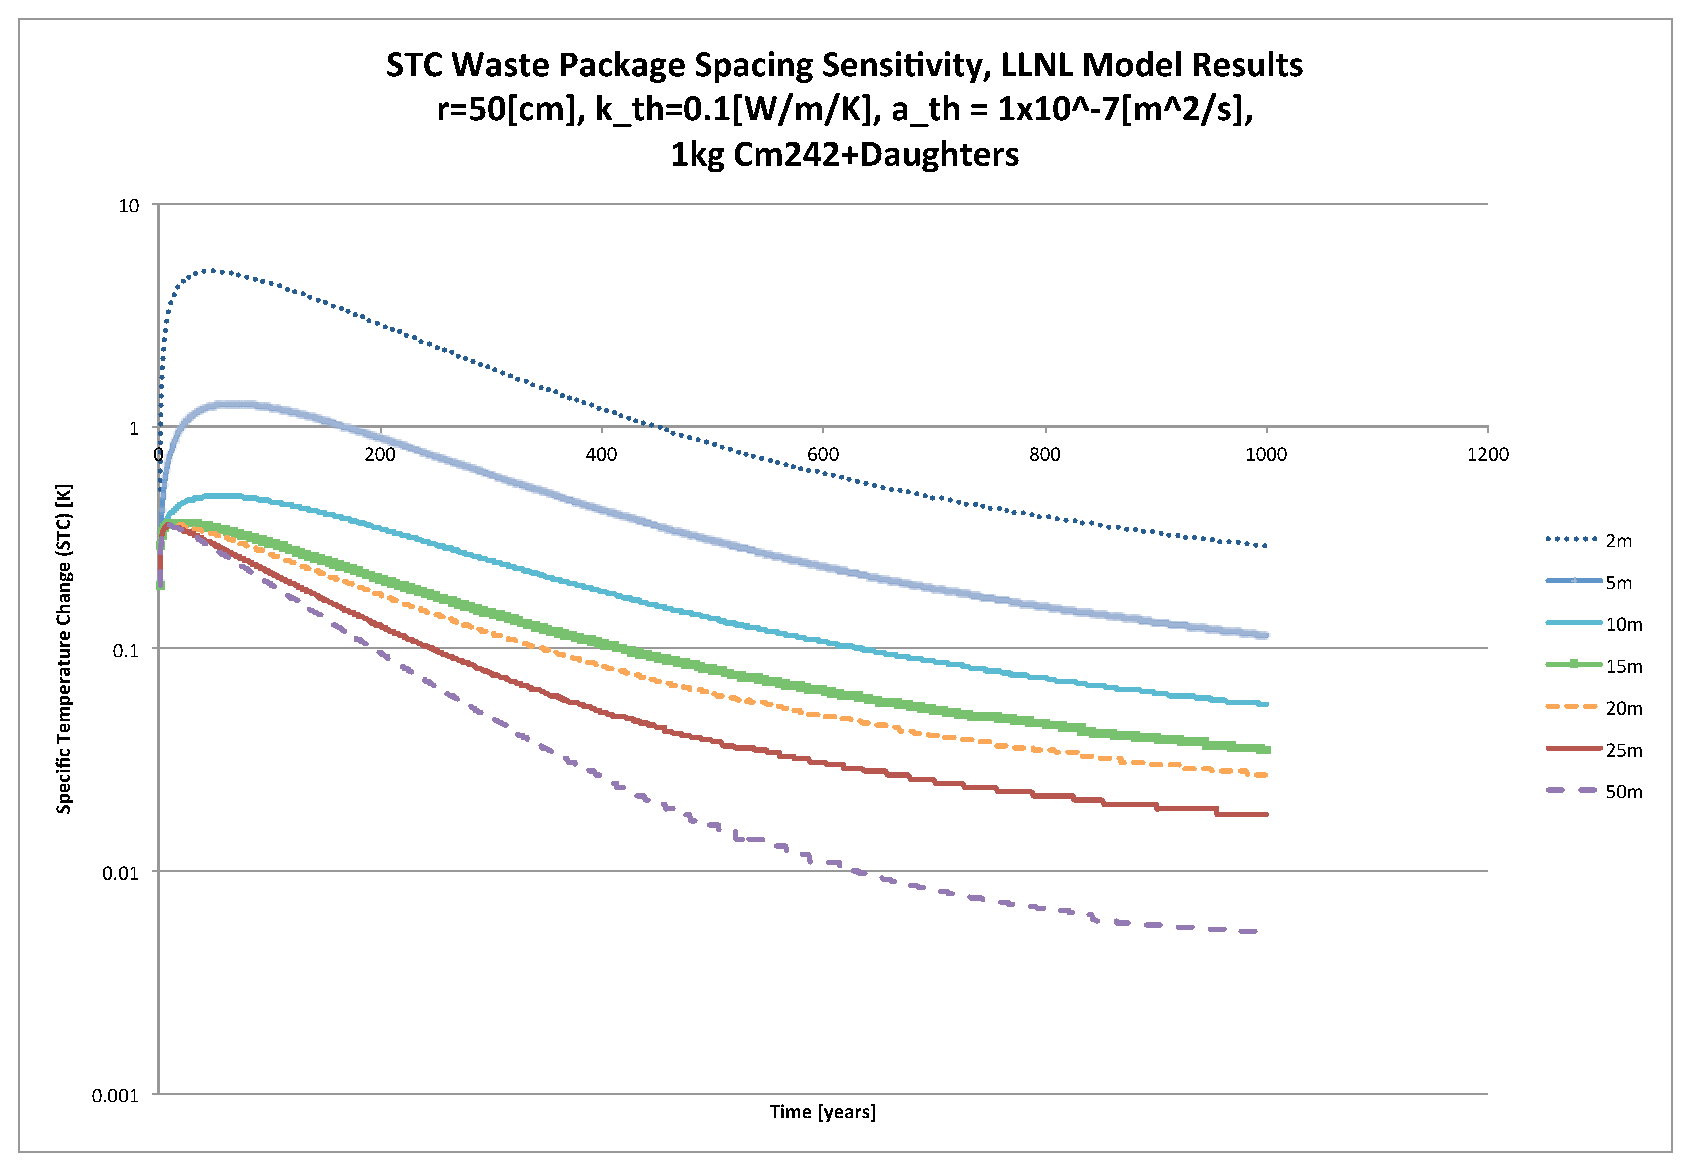
\includegraphics[height=0.7\textheight]{./thermal_demonstration/spacing/Cm242spacing_sens.eps}
\end{center}
\caption[$K_{th}$ Sensitivity to $s$]{Increased waste package 
spacing decreases areal thermal energy deposition 
(here represented by STC) in the near field (here $r_{calc} = 0.5m$).}
\label{fig:Cm242spacing_sens}
\end{figure}
}
\end{frame}


\begin{frame}[ctb!]
\frametitle{LLNL Model Limiting Radius Sensitivity}
\footnotesize{
The location of the limiting radius has a strong effect on the 
waste package loading limit, for a fixed limiting temperature. 
\begin{figure}[htbp!]
\begin{center}
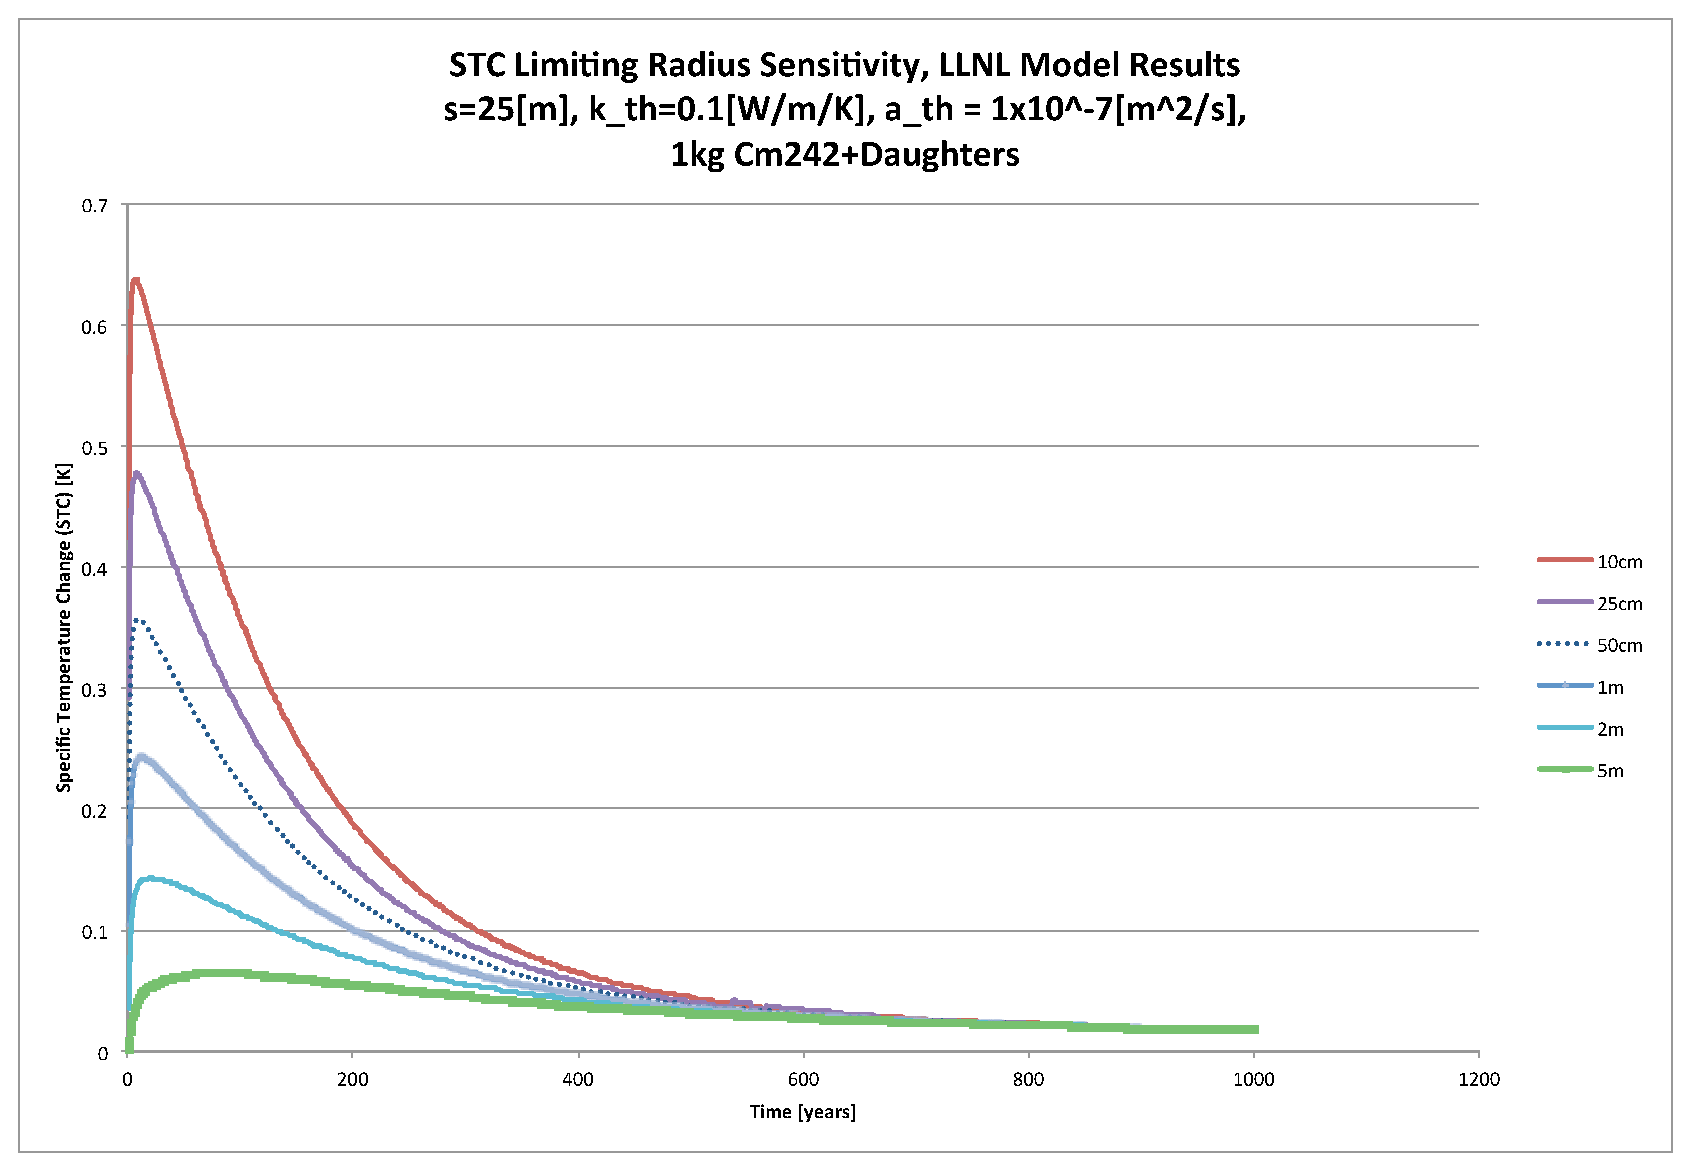
\includegraphics[height=0.7\textheight]{./thermal_demonstration/spacing/Cm242r_lim_sens.eps}
\end{center}
\caption[$K_{th}$ Sensitivity to $r_{lim}$]{Increased limiting radius 
decreases thermal energy deposition contributing to the thermal limit
(here represented by STC).}
\label{fig:Cm242r_lim_sens}
\end{figure}
}
\end{frame}

\begin{frame}[ctb!]
\frametitle{Cyder Spacing and Limiting Radius Sensitivity}
\footnotesize{
The thermal diffusivity was compared both with the 
spacing between waste packages and the limiting radius. 

\begin{figure}[htbp!]
\begin{center}
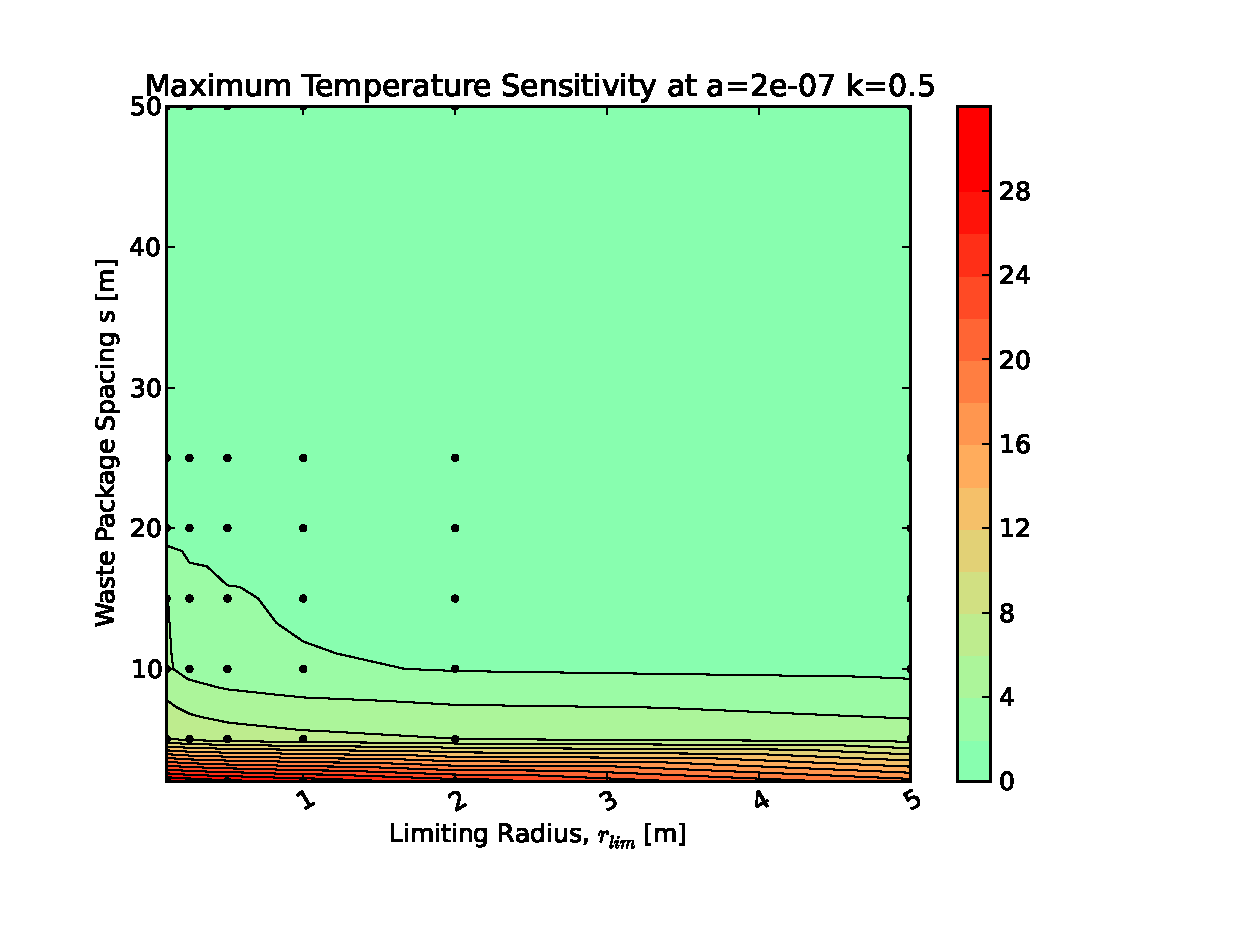
\includegraphics[height=0.7\textheight]{./thermal_demonstration/spacing/rs.eps}
\end{center}
\caption[$\alpha_{th}$ vs. $r_{lim}$ Sensitivity in Cyder]
{Cyder results agree with 
those of the LLNL model. The importance of the limiting radius decreases with 
increased $K_{th}$. The above example thermal profile results from 10kg of 
$^{242}Cm$}
\label{fig:rs}
\end{figure}
}
\end{frame}
